\section{Overview}\index{EP}
Now that we know how the basic elements of a particle physics detector work, let's see how we can use them to identify which types of particles produce which signals in our detector.  
We will consider specifically the CMS detector, but virtually all collider detectors use similar identification criteria.

Particle identification is done using a massive piece of software, written by hundreds of physicists scattered all over the world, called CMSSW.  What does this code do?

When a particle enters a detector element, some sort of detectable signal, usually charge, is made.  This charge is measured, usually using something called an ADC or analog-to-digital converter.  A number in binary (a number in base 2 number system) is produced and stored. For interesting events, every detector element (and there are millions of them, Figure ~\ref{fig:count} shows the channel count by subdetector) that has a reading above some threshold must be pulled from the detector electronics, along with an ID number that will identify which detector element the number came from, assembled into an organized structure in computer memory, and written to some storage media (perhaps computer disk).  

\begin{figure}[ht]
\centering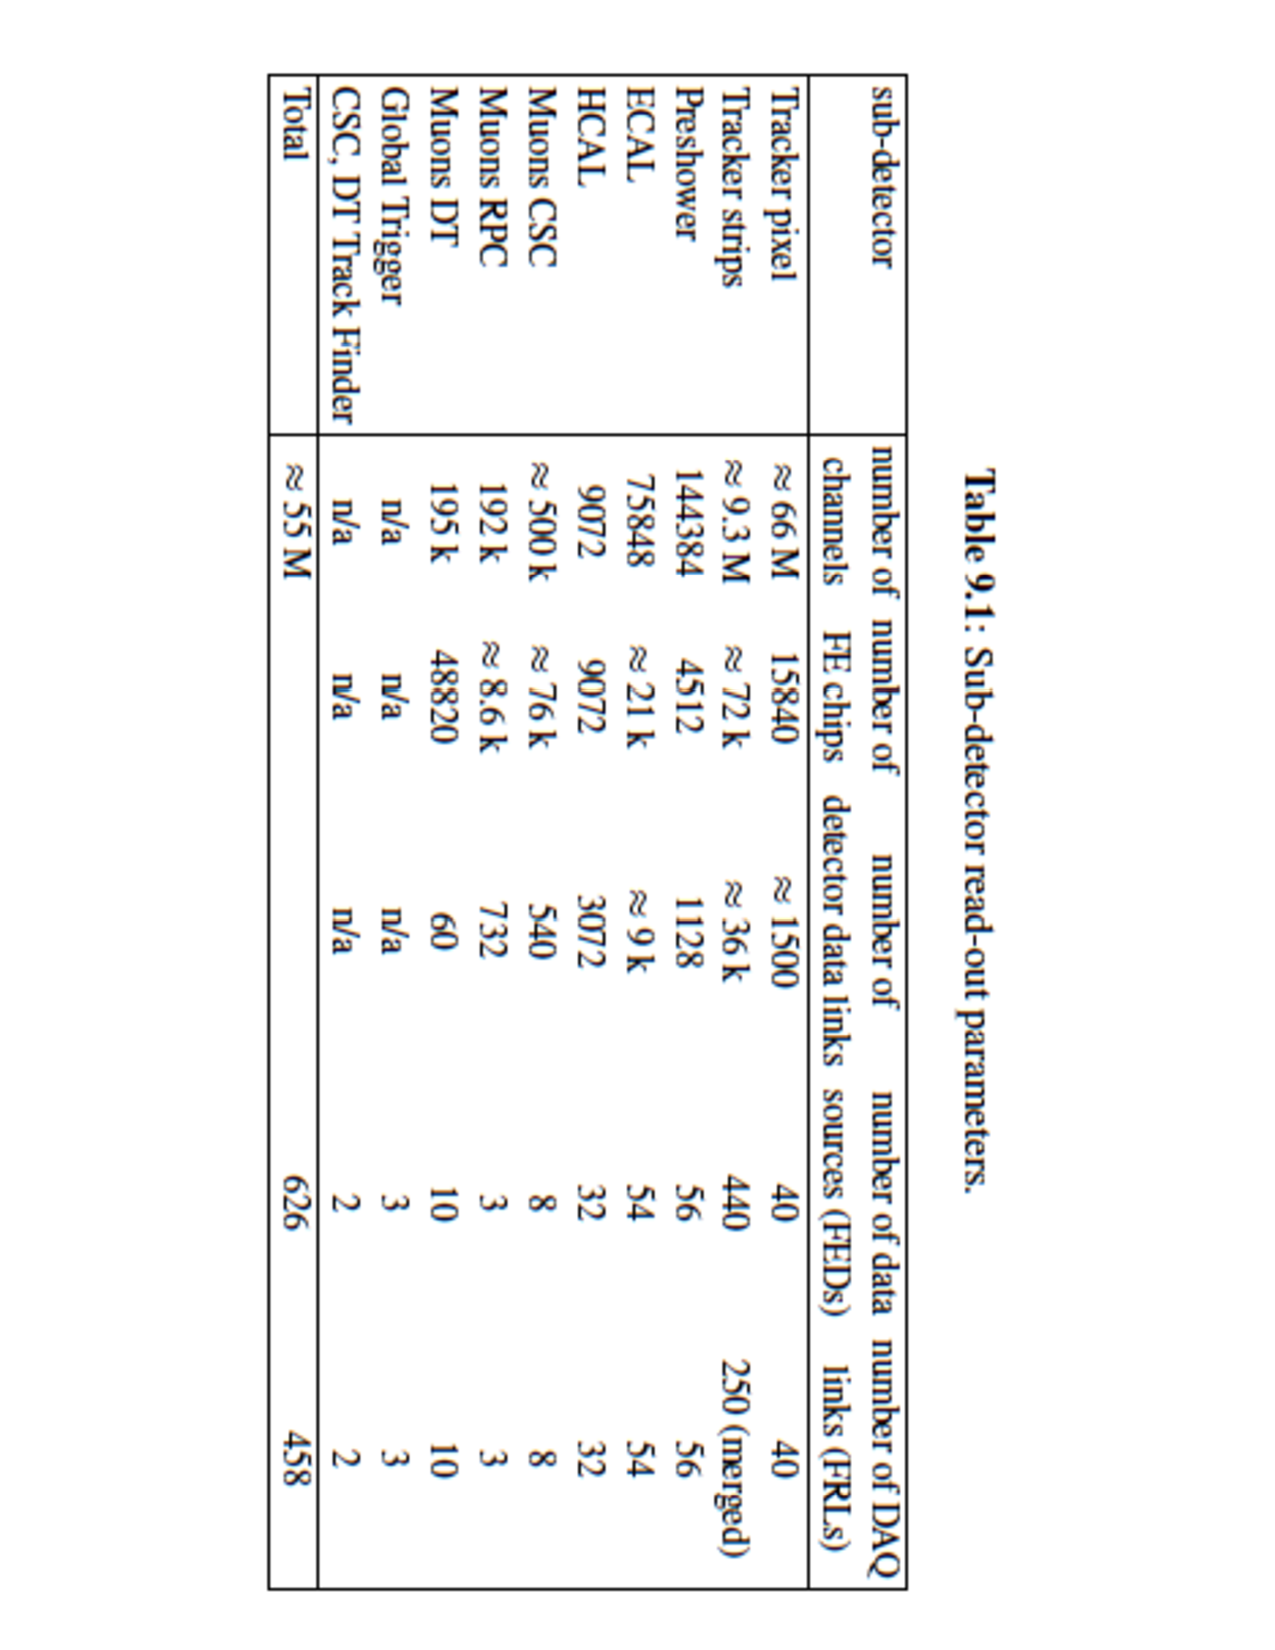
\includegraphics[scale=0.6,angle=90]{./particleID/Pictures/channelcount.pdf}
\caption{Channel count for the CMS detector by subdetector}
\label{fig:count}
\end{figure} 

CMSSW takes all these 0's and 1', uses calibration data to convert these to energies, times, or whatever is relevent for that subdetector. Once this is done,   complex computer algorithms are run on this information to figure out which particles were produced.  

We describe below some of the types of algorithms that are used in this code.


Consider the slice of the CMS detector show in Figure \ref{fig:pid1} as viewed in the r-$\phi$ plane: 
\begin{figure}[h]
\centering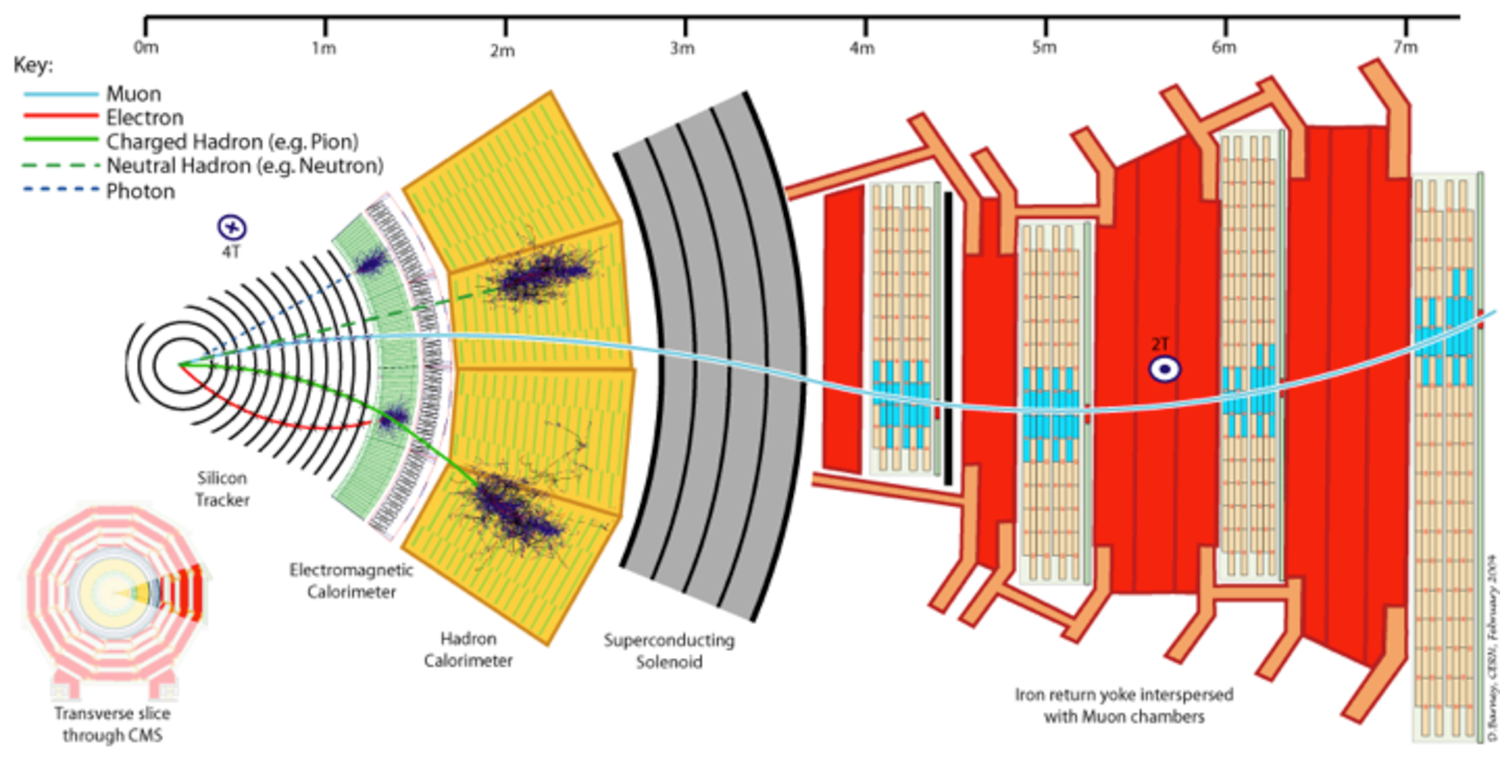
\includegraphics[scale=0.6]{./particleID/Pictures/fig1.pdf}
\caption{A slice of the CMS detector as viewed in the r-$\phi$ plane with typical signals produced by various types of particles.}
\label{fig:pid1}
\end{figure} 
\\*
The collision point in the figure above is indicated by the convergence of the solid red, green, and blue lines and the dashed green and blue lines. These represent particles created at a common point when a collision occurs. Outward from the collision point, we have the silicon tracker, the electromagnetic calorimeter, the hadronic calorimeter, the solenoid magnet, and the muon trackers embedded in the ``return iron'' for the magnet (as you know, magnetic field lines must form closed loops. They cannot have a beginning or an end, until we discover the mythical magnetic monopole. The magnetic field lines that form the field inside the magnet must continue out one end, loop around, and come back to come in the other end. The ``return yoke'', made of iron, guides these field lines so that they do not interfere with the detector electronics).  
\\
\\
\noindent
Let's see how we can use the information from these detectors to identify particles.
\section{Photons}
In Figure~\ref{fig:pid1}, the photon is indicated by the dashed blue line.  Photons are electrically neutral so they do not produce a signal in any of the trackers. Because they can interact with nuclei in the material via the long range electromagnetic interaction of pair production, they shower quickly upon impact, and the shower is almost completely contained in the EM calorimeter.
\section{Electrons}
In figure \ref{fig:pid1}, the electron is indicated by the solid red line. Their signature is similar to that of a photon (although their initiating interaction is bremsstrahlung, not pair production), but there is an associated charged track.
\section{Muons}
In figure \ref{fig:pid1}, the muon is indicated by the solid blue line. Muons are charged and so they produce a track in the inner tracker. Muons predominantly lose energy by exciting or ionizing the electrons in the material. Because of this, they lose energy slowly. They can pass through the calorimeters, losing only about a GeV of energy.  They are the only charged particle that can do this.  Tracking chambers (gas-based) outside the calorimeters, embedded in the return yoke, are used to indicate a penetrating particle.
\section{Hadrons}
In figure \ref{fig:pid1}, a charged hadron is indicated by the solid green line and a neutral hadron is indicated by the dashed green line. Hadrons interact with nuclei via the short-range strong force (QCD) interaction. Therefore, their shower will typically start deeper into the calorimeter and it will take more material to completely convert the kinetic energy of the hadron into energy of the material. The shower needs the thicker combined electromagnetic and hadronic calorimeter to contain it. Charged and neutral hadrons are distinguished by the presence of a track in the tracker.
\section{Event displays}
While we wait for physics results, complex computer algorithms are used to find the particles.  The human mind also has very powerful identification capabilities - physicists use event displays to look at the information and identify particles ``by hand''. In the vast majority of the cases, when the human ``scanner'' and the computer algorithm disagree, the human is right.  It is important to verify computer algorithms and search for bugs by comparing the results from ``scanning'' to the computer based results.
\\*
\\*
Typically two types of displays are used. One has a cartoon of the detector with symbols to denote energy deposits.  The results from the computer identification algorithm are usually superimposed.  An example is shown in figure ~\ref{fig:pid2}. You can see the cartoon of the muon chambers in pink. The tracks reconstructed in the tracker are shown as green lines. Energies in the EM calorimeter are shown as red blobs and in the HAD calorimeter as blue blobs. Their shape reflects the segmentation of the electrical readouts of the detector information.
\begin{figure}[h]
\centering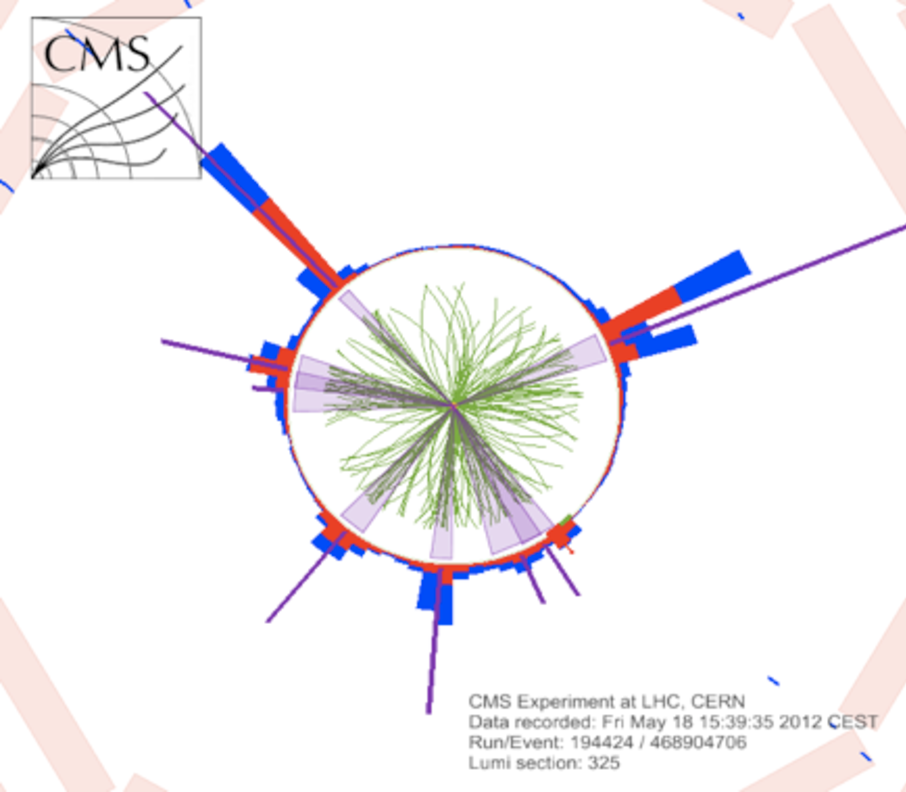
\includegraphics[scale=0.5]{./particleID/Pictures/fig2.pdf}
\caption{An event display from the CMS experiment}
\label{fig:pid2}
\end{figure}
\\*
Another kind of event display is called a ``Lego'' plot (named after the Children's toy), and it is the most common way of displaying calorimeter information.  This kind of display is a 3-D plot with two of the axes being the polar angle and the pseudorapidity, and the ``z'' axes being the energy deposited in the calorimeter at that location. Colors indicate which part of the energy was deposited in the electromagnetic and which in the hadronic calorimeter. An example is shown in figure \ref{fig:pid3}, along with the corresponding regular display.
\begin{figure}[h]
\centering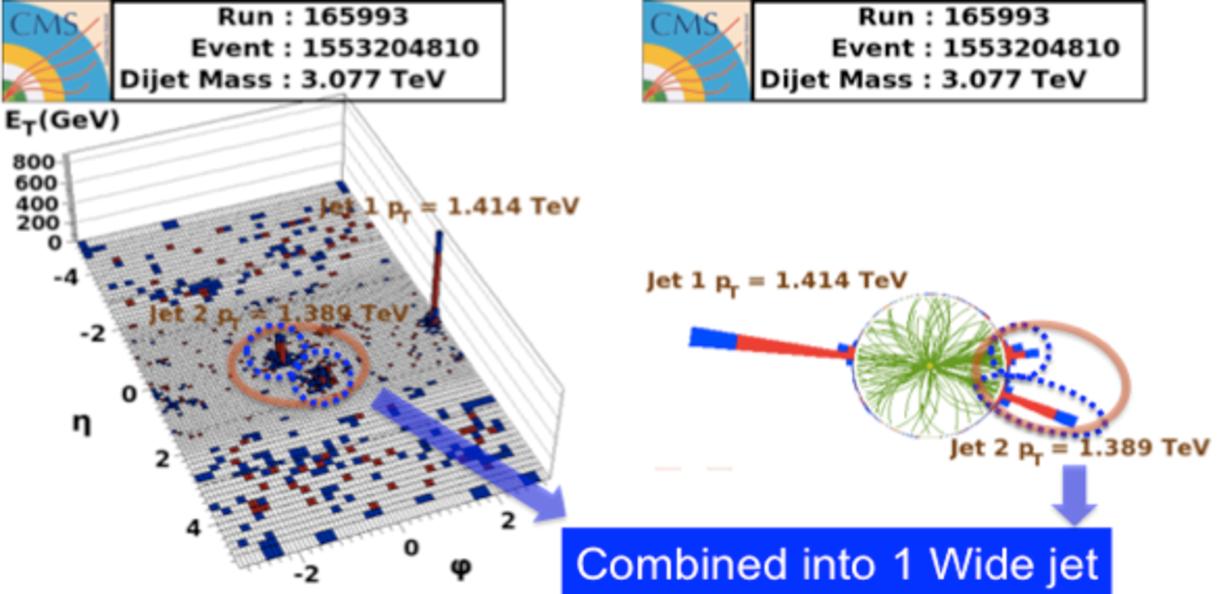
\includegraphics[scale=0.5]{./particleID/Pictures/fig3.pdf}
\caption{A lego display along wih the corresponding regular display of an event taken with the CMS detector.}
\label{fig:pid3}
\end{figure}

\section{Neutrinos}
There is one particle that is so weakly interacting that does not produce a signal in our detector. However, we can infer its presence using conservation of momentum. The momentum of the beams is along the z-axis. This means that the total initial momentum can only be along the z direction, and the initial component of momentum transverse to the beam axis must be zero. By conservation of momentum, the final component of momentum transverse to the beam axis must also be zero.  So, if we sum the transverse momenta of all observed particles, the sum of the momenta of all unobserved particles must be equal in magnitude but opposite in direct to this, so that the sum is zero.  Usually this can be attributed to a single neutrino. Figure \ref{fig:pid4} shows the particles projected in the transverse plane. Since the observed momenta obviously cannot sum to zero, we infer that a neutrino was present in the event.
\begin{figure}[h]
\centering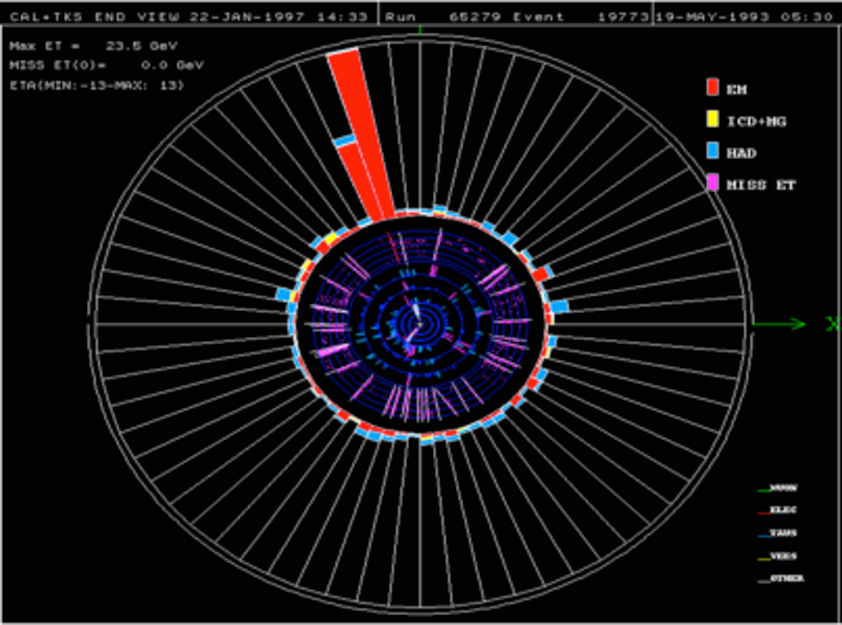
\includegraphics[scale=0.4]{./particleID/Pictures/fig4.pdf}
\caption{\small An event display from the D0 detector at the FNAL Tevatron. The red blob represents energy in the EM calorimeter. Since it has an associated track, it is identified as an electron. This is probably the decay of a W boson to an electron and a neutrino. The neutrino is assumed to have a transverse momenta that is equal in magnitude and opposite in direction to the sum of the momenta of all other particles in the event.}
\label{fig:pid4}
\end{figure}
\\*
This was, in fact, how Fermi discovered the neutrino - by considering conservation of momentum in certain radioactive decays of nuclei (beta decays). 

\section{Quarks/Gluons (jets)}
As you may have noticed from the event displays shown above and from the one shown below, hadrons tend to come in clusters called ``jets''. These jets are the signatures of quarks and gluons, that ``fragment'' into a number of hadrons - typically 10 charged hadrons and 5 neutral, but with statistical fluctuations with the rms that occurs for any thing produced randomly that can counted ($\sqrt{N}$).
\\*
\\*
Generally, the individual momenta of the hadrons are not that interesting in our studies of forces and particles; what we really want to know is the momenta of the quarks and gluons that created them. To find this, we just have to figure out which hadrons came from the same ``parent'' particle and (by conservation of momentum), sum their momentum to get the parent momenta.
\\*
\noindent
However, because gluons can be radiated off of quark or gluon jets, and the resulting jets are very close to each other (among other more fundamental but technical reasons), it is not trivial to figure out which hadrons belong together, which came from the same ``parent''.
\\*
To do this,``jet finding algorithms'' have been developed. Figure ~\ref{fig:pid5} shows how four different algorithms divided up the calorimeter energies into ``jets''.
\begin{figure}[h]
\centering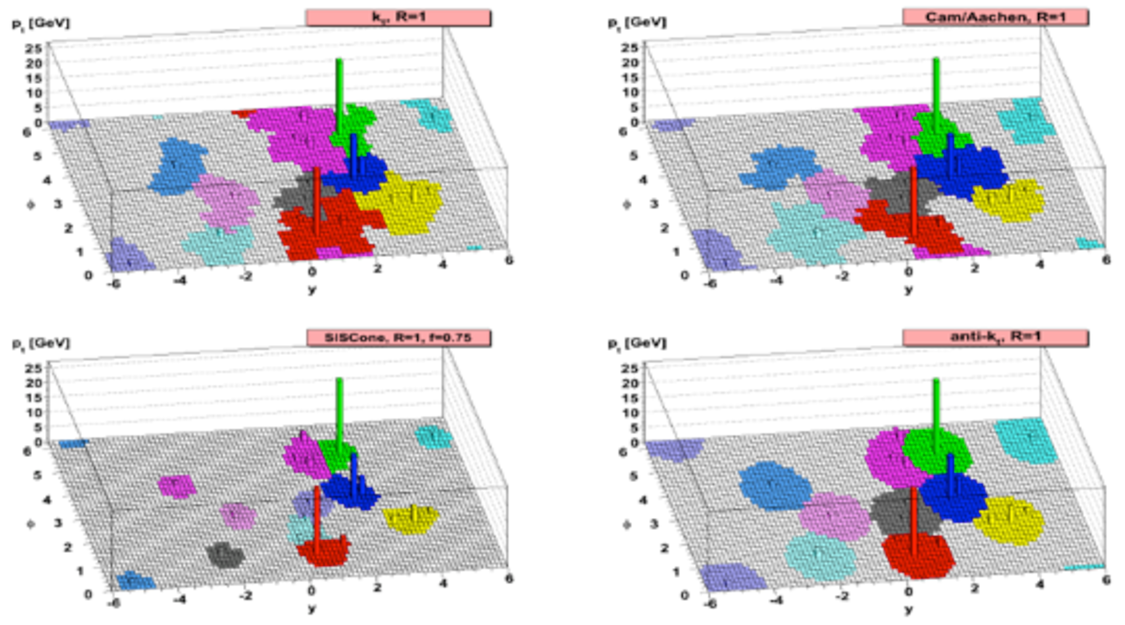
\includegraphics[scale=0.6]{./particleID/Pictures/fig5.pdf}
\label{fig:pid5}
\end{figure}
\\*
\noindent
Let's look at one of these algorithms (which is implemented in CMSSW and is the most popular), which you will easily be able to imagine as code (and which clearly can not be handled any other way). This algorithm is called the anti-$k_{T}$ algorithm (don't ask) with cone-parameter R. R is typically chosen to be 0.4.
\\*
\\*
\begin{itemize}
\item For all possible pairs of particles in an event (particle i and particle j), $d_{ij}$ = min(p$_{Ti}$$^{-2}$, p$_{Tj}$$^{-2}$)$\Delta\frac{R_{ij}^{2}}{R^{2}}$ where $R=\sqrt{(\Delta\phi)^{2}+(\Delta\eta)^{2}}$ and $\Delta\phi$ is the difference in azimuthal angles between the two particles and $\Delta\eta$ is the difference in their pseudorapidities.
\item For each particle, calculate $d_{iB}$=$p_{T}^{-2}$
\item Take the minimum of all $d_{ij}s$ and $d_{iB}s$
\item If the smallest is a $d_{ij}$, combine them into a single particle by adding their 4-momenta, add this particle to the list of particles and remove the two individual particles.  Go back to the beginning.
\item If it is a $d_{iB}$, call it a jet, remove the corresponding particle from the particle list, add it to the jet list, and go back to the beginning.
\item Stop when there are no particles left in the particle list.
\end{itemize}
\newpage
\noindent
\vspace{.2cm} 
\begin{minipage}{0.7\textwidth} 
\begin{framed}
%\vspace{.1cm}
\begin{exercise}
%\begin{frshaded}
%\fcolorbox{\bordercolor}{\backgroundcolor} 
{Look at the event displays found at xxx. For each event display, tell us what kind of particles you see}
\end{exercise}
%\end{frshaded}
%\vspace{.1cm}
\end{framed} 
\end{minipage}
\vspace{.2cm}
\\*
\vspace{.2cm} 
\begin{minipage}{0.7\textwidth} 
\begin{framed}
%\vspace{.1cm}
\begin{exercise}
%\begin{frshaded}
%\fcolorbox{\bordercolor}{\backgroundcolor} 
{The root file found in https://github.com/saraheno/jetclusteringexercise  has particle 4-momenta for particles reconstructed for a bunch of events. Write code to cluster these into jets. Use the anti-$k_{T}$ cone algorithm with cone parameter 0.4. Make a histogram showing the $p_{T}$ spectra of the jets.}
\end{exercise}
%\end{frshaded}
%\vspace{.1cm}
\end{framed} 
\end{minipage}
\vspace{.2cm}

\section{Further Reading}
\noindent
$\cdot$ \url{http://www.sciencedirect.com/science/article/pii/S0168900211005419}
